To map a SOM, the main principle is to initiate a learning process with a significative dataset, using the decreasing function \glspl{exp-decay} applied on the learning rate and on the radius of neighbourhood influence in relation with the number of iteration, defined by $\alpha_{(t)} = \alpha_0 e^{(-t/T)}$ with $\alpha_0$ as the initial value and $T=n/|ln(\alpha_n/\alpha_0)|$ with $n$ as the number of iterations. 

\bigskip

See code on the Annex \ref{ann:color} on page \pageref{ann:color}.

\begin{figure}[htbp]
\begin{center}
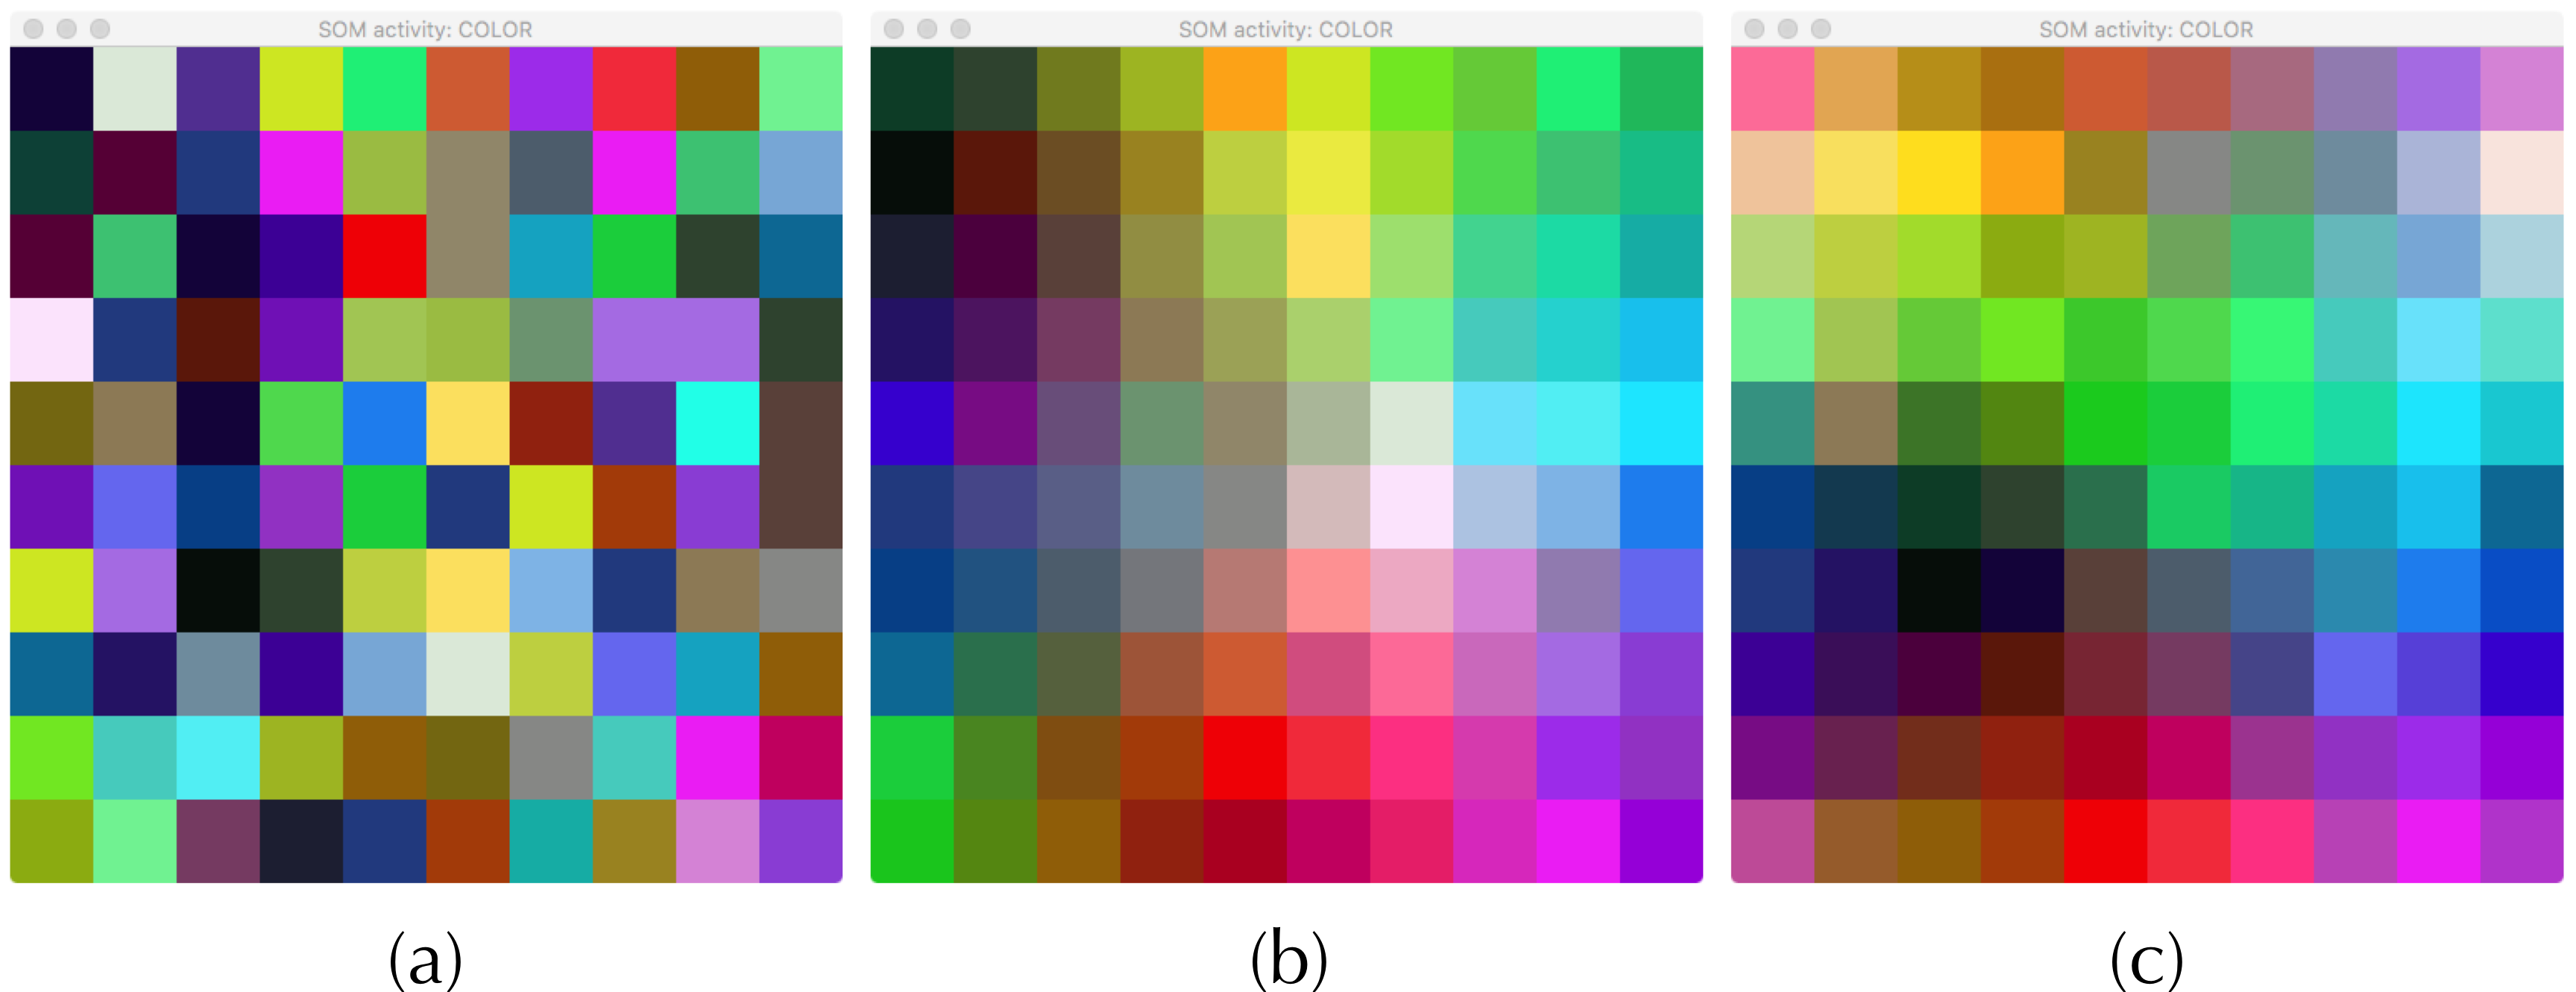
\includegraphics[width=\columnwidth]{2322}
\caption{(a) A map of 100 neurons initialised with random colors. (b) The same map after 3000 iteration. (c) Same process than (b) but with modulo.}
\label{fig:ex1}
\end{center}
\end{figure}

Note that the illustration (c) on figure \ref{fig:ex1} the modulo considers each neuron as the middle of the map. Thus, a more accurate representation of this mapping takes the form of a `donut' (i.e. a torus).